% Architecture of the modular-nft-erc721 repository.
% Render: tectonic docs/architecture.tex  (then convert the PDF to PNG)
\documentclass[tikz,border=8pt]{standalone}
\usepackage{mathptmx}
\usepackage[T1]{fontenc}
\usepackage[scaled=0.9]{helvet}
\usetikzlibrary{arrows.meta,fit}
\begin{document}
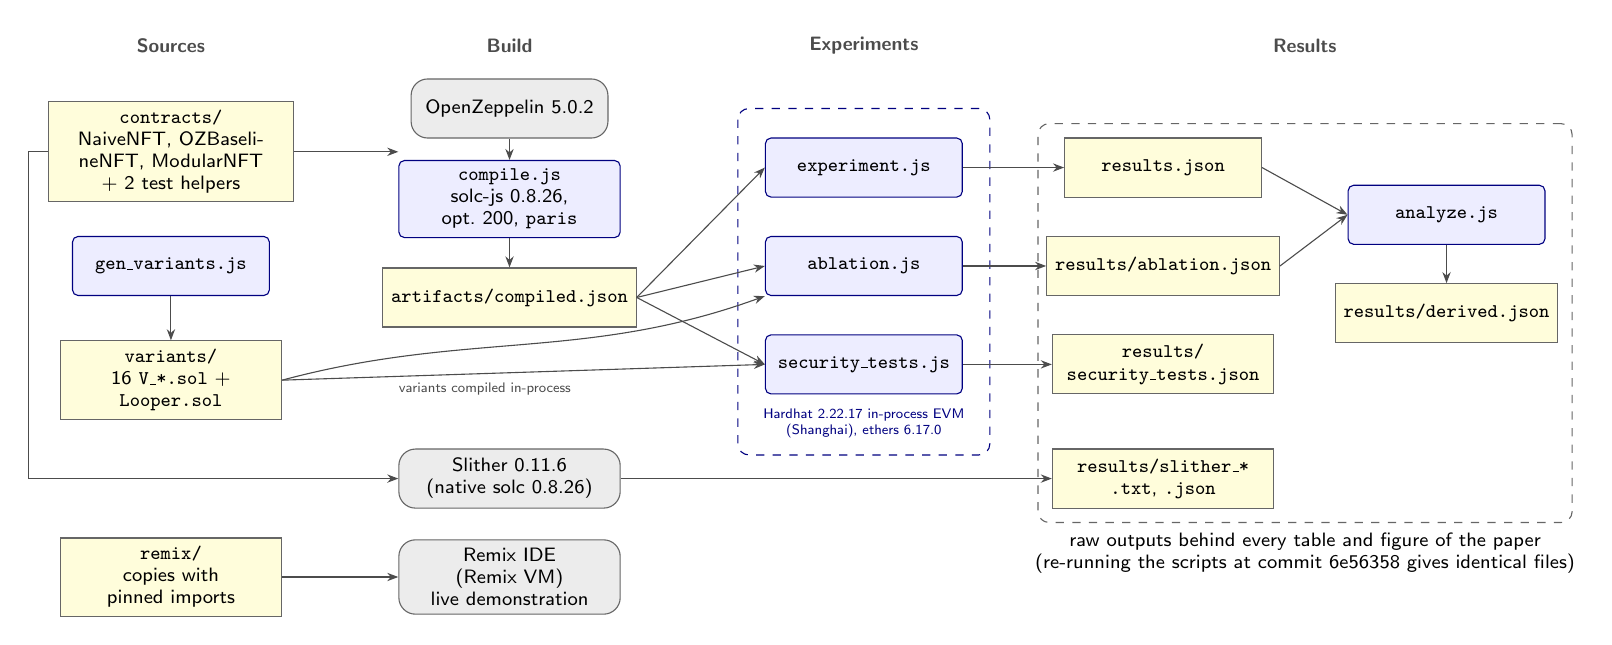
\begin{tikzpicture}[font=\sffamily\scriptsize,
 script/.style={draw=blue!50!black,fill=blue!7,rounded corners=2pt,align=center,minimum height=0.75cm,minimum width=2.5cm,inner sep=3pt},
 file/.style={draw=black!60,fill=yellow!14,align=center,minimum height=0.75cm,minimum width=2.5cm,inner sep=3pt},
 tool/.style={draw=black!60,fill=gray!15,rounded corners=6pt,align=center,minimum height=0.75cm,minimum width=2.5cm,inner sep=3pt},
 arr/.style={-{Stealth[length=4pt]},black!70},
 lbl/.style={font=\sffamily\scriptsize\bfseries,text=black!70}]
% column headings
\node[lbl] at (0,1.35) {Sources};
\node[lbl] at (4.3,1.35) {Build};
\node[lbl] at (8.8,1.35) {Experiments};
\node[lbl] at (14.4,1.35) {Results};
% sources
\node[file,text width=2.9cm] (con) at (0,0) {\texttt{contracts/}\\NaiveNFT, OZBaselineNFT, ModularNFT + 2 test helpers};
\node[script] (gen) at (0,-1.45) {\texttt{gen\_variants.js}};
\node[file,text width=2.6cm] (var) at (0,-2.9) {\texttt{variants/}\\16 \texttt{V\_*.sol} + \texttt{Looper.sol}};
\node[file,text width=2.6cm] (rmx) at (0,-5.4) {\texttt{remix/}\\copies with pinned imports};
\draw[arr] (gen) -- (var);
% build
\node[tool] (oz) at (4.3,0.55) {OpenZeppelin 5.0.2};
\node[script,text width=2.6cm] (cmp) at (4.3,-0.6) {\texttt{compile.js}\\solc-js 0.8.26, opt.\ 200, \texttt{paris}};
\node[file] (art) at (4.3,-1.85) {\texttt{artifacts/compiled.json}};
\node[tool,text width=2.6cm] (sl) at (4.3,-4.15) {Slither 0.11.6\\(native solc 0.8.26)};
\node[tool,text width=2.6cm] (rid) at (4.3,-5.4) {Remix IDE (Remix VM)\\live demonstration};
\draw[arr] (oz) -- (cmp);
\draw[arr] (con.east) -- (cmp.west |- con.east);
\draw[arr] (cmp) -- (art);
\draw[arr] (con.west) -- ++(-0.25,0) |- (sl.west);
\draw[arr] (rmx) -- (rid);
% experiments inside the EVM
\node[script] (exp) at (8.8,-0.2) {\texttt{experiment.js}};
\node[script] (abl) at (8.8,-1.45) {\texttt{ablation.js}};
\node[script] (sec) at (8.8,-2.7) {\texttt{security\_tests.js}};
\draw[draw=blue!50!black,dashed,rounded corners=4pt] (7.2,0.55) rectangle (10.4,-3.85);
\node[font=\sffamily\tiny,align=center,text=blue!50!black] at (8.8,-3.45) {Hardhat 2.22.17 in-process EVM\\(Shanghai), ethers 6.17.0};
\draw[arr] (art.east) -- (exp.west);
\draw[arr] (art.east) -- (abl.west);
\draw[arr] (art.east) -- (sec.west);
\draw[arr] (var.east) to[out=15,in=200] (abl.south west);
\draw[arr] (var.east) -- node[pos=0.42,below,font=\sffamily\tiny] {variants compiled in-process} (sec.west);
% results
\node[file] (rj) at (12.6,-0.2) {\texttt{results.json}};
\node[file] (aj) at (12.6,-1.45) {\texttt{results/ablation.json}};
\node[file,text width=2.6cm] (sj) at (12.6,-2.7) {\texttt{results/}\\\texttt{security\_tests.json}};
\node[script] (ana) at (16.2,-0.8) {\texttt{analyze.js}};
\node[file] (dj) at (16.2,-2.05) {\texttt{results/derived.json}};
\node[file,text width=2.6cm] (so) at (12.6,-4.15) {\texttt{results/slither\_*}\\\texttt{.txt}, \texttt{.json}};
\draw[arr] (exp) -- (rj);
\draw[arr] (abl) -- (aj);
\draw[arr] (sec) -- (sj);
\draw[arr] (rj.east) -- (ana.west);
\draw[arr] (aj.east) -- (ana.west);
\draw[arr] (ana) -- (dj);
\draw[arr] (sl.east) -- (so.west);
% what the results feed
\node[draw=black!60,dashed,rounded corners=4pt,fit=(rj)(sj)(so)(dj)(ana),inner sep=5pt] (res) {};
\node[font=\sffamily\scriptsize,align=center,anchor=north] at (res.south) {raw outputs behind every table and figure of the paper\\(re-running the scripts at commit 6e56358 gives identical files)};
\end{tikzpicture}
\end{document}
